%! Author = Matthias
%! Date = 03.11.2020

% Preamble
\documentclass[11pt]{article}

% Packages
\usepackage{amsmath}
\usepackage{german}
\usepackage{gensymb}
\usepackage{listings}
\usepackage{xcolor}
\usepackage{graphicx}
\usepackage{float}
% Document
\begin{document}

    \definecolor{codegreen}{rgb}{0,0.6,0}
    \definecolor{codegray}{rgb}{0.5,0.5,0.5}
    \definecolor{codepurple}{rgb}{0.58,0,0.82}
    \definecolor{backcolour}{rgb}{0.95,0.95,0.92}


    \lstdefinestyle{mystyle}{
    backgroundcolor=\color{backcolour},
    commentstyle=\color{codegreen},
    keywordstyle=\color{magenta},
    numberstyle=\tiny\color{codegray},
    stringstyle=\color{codepurple},
    basicstyle=\ttfamily\footnotesize,
    breakatwhitespace=false,
    breaklines=true,
    captionpos=b,
    keepspaces=true,
    numbers=left,
    numbersep=5pt,
    showspaces=false,
    showstringspaces=false,
    showtabs=false,
    tabsize=2
    }
    \lstset{style=mystyle}

\section{Haus"ubung 2}\label{sec:h2}
    Unsicherheitsfaktoren: $k_{r} = k_{l} = 0.001$\newline
    Radabstand: d = 20cm\newline
    Meine Angaben (Aufgabe 8):\newline
    Startposition: x = 0, y = 0, $\theta = 60\degree$\newline
    Pfad: 5 Schritte mit jeweils 15 cm vorw"arts, ein Schritt mit Drehung um $\pi/2$, dann 5 Schritte mit jeweils 15 cm vorw"arts.\newline
    Code:\newline
Funktion f"ur die Berechnung von $G_{s}$:
\lstinputlisting[language=Octave]{Jakobi_s.m}
Funktion f"ur die Berechnung von $G_{p}$
\lstinputlisting[language=Octave]{Jakobi_p.m}
Funktion f"ur die Berechnung der $\Delta s$ der R"ader:
\lstinputlisting[language=Octave]{Get_wheel_deltas.m}
Funktion f"ur die Berechnung der Kovarianzmatrix der R"ader:
\lstinputlisting[language=Octave]{Covariance_drive.m}
Funktion f"ur die Berechnung der n"achsten Kovarianzmatrix:
\lstinputlisting[language=Octave]{Covar_next.m}
Helferfunktion, die anhand der Eingabewerte alle n"otigen Vorberechnungen (Jakobimatrizen, etc.) mit den entsprechenden Funktionen ausf"uhrt und dann die n"achste Kovarianzmatrix mit Covar\_next berechnet:
\lstinputlisting[language=Octave]{Calc_next_covar.m}
Funktion, die die n"achste Pose des Roboters berechnet:
\lstinputlisting[language=Octave]{Calc_new_pose.m}
Funktion, die bei gleichbleibenden Eingabewerten eine beliebige Anzahl Schritte hintereinander berechnet und plottet:
\lstinputlisting[language=Octave]{Draw_Loop.m}
Skript, das die Aufgabe 8 mit hilfe der anderen Funktionen berechnet:
\lstinputlisting[language=Octave]{loop_calc.m}
    Hier noch das anhand dieses Codes ermittelte Bild:
    \begin{figure}[H]
        \centering
        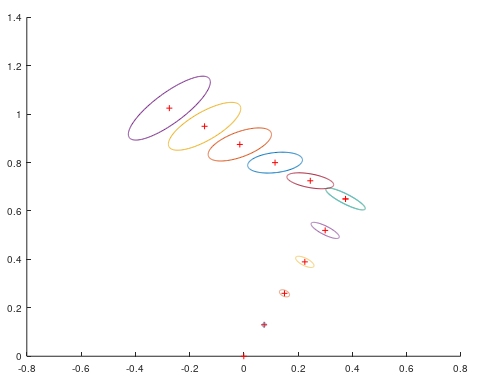
\includegraphics[width=6cm]{aufgabeResultat.png}
        \caption{Mimicry flowchart}
        \label{fig:result}
    \end{figure}

\end{document}